\chapter{突变与遗传变异}\label{ch:g11:mutations}

一个孩子出生时全无色素——白发、苍白的皮肤、
眼睛无法耐受强光——其父母双方都是普通人，
家族中没有此病史。一个从未
接触过抗生素的细菌菌落，在一亿个\omterm{def:g10:cells-common-unit:cell}{细胞}中含有少数
已能抵抗它。一位园丁发现一丛玫瑰中的一根枝条
开出不同颜色的花。在每种情形下，一段 \omterm{def:g10:universal-dna:information}{DNA} 序列
在某一\omterm{def:g10:cells-common-unit:cell}{细胞}中发生一次改变；每种情形中，该改变
此后都被忠实地复制。本章讨论这些改变：它们
是什么、从何而来、\omterm{def:g10:cells-common-unit:cell}{细胞}如何限制它们，以及为何生命
依赖于它们永不停歇地发生。

\section{什么是突变}

\begin{definition}[突变]\label{def:g11:mutations:mutation}
称\emph{突变}\index{突变}为 \omterm{def:g10:universal-dna:information}{DNA} 分子中\omterm{def:g10:universal-dna:nucleotide}{核苷酸}序列的改变，
并传递给发生该改变的
\omterm{def:g10:cells-common-unit:cell}{细胞}的后代。最常见的是\emph{点突变}，
即影响一个或几个\omterm{def:g10:universal-dna:nucleotide}{核苷酸}的突变：
\begin{itemize}
  \item \emph{替换}：一个\omterm{def:g10:universal-dna:nucleotide}{核苷酸}被另一个替换；
  \item \emph{插入}：增加一个或多个\omterm{def:g10:universal-dna:nucleotide}{核苷酸}；
  \item \emph{缺失}：去掉一个或多个\omterm{def:g10:universal-dna:nucleotide}{核苷酸}。
\end{itemize}
较大的改变——一段被重复、倒位或移位的片段，或整条
\omterm{def:g11:cell-cycle-mitosis:chromosome}{染色体}被获得或丢失——同样属于突变。
\end{definition}

\begin{omfigure}
\begin{tikzpicture}[font=\small\ttfamily]
  \tikzset{seq/.style={anchor=west}}
  \node[seq] at (0,0) {原始\phantom{甲}\ \ \ \ \ ATG GCT TAC GGA TCC};
  \node[seq] at (0,-0.8) {替换\ \ \ \ \ \ \ \ ATG GCT T\textcolor{omThm}{\textbf{G}}C GGA TCC};
  \node[seq] at (0,-1.6) {插入\ \ \ \ \ \ \ \ ATG GCT TA\textcolor{omThm}{\textbf{A}} CGG ATC C};
  \node[seq] at (0,-2.4) {缺失\ \ \ \ \ \ \ \ ATG GCT T\textcolor{omThm}{\textbf{\_}}C GGA TCC};
  \node[seq, font=\small] at (7.9,-0.8) {改变一个字母};
  \node[seq, font=\small] at (7.9,-1.6) {增加一个字母：其后序列整体移位};
  \node[seq, font=\small] at (7.9,-2.4) {删除一个字母：其后序列整体移位};
\end{tikzpicture}

{\small 同一序列的三个点\omterm{def:g11:mutations:mutation}{突变}（字母按三个一组
分组，其原因在
\cref{ch:g11:gene-expression}中说明）。替换只改变一个位置；
插入或缺失会使其后的全部序列移位。}
\end{omfigure}

\begin{proposition}[突变发生在何处，又影响谁]\label{prop:g11:mutations:where}
发生在体\omterm{def:g10:cells-common-unit:cell}{细胞}中的\omterm{def:g11:mutations:mutation}{突变}（\emph{体\omterm{def:g10:cells-common-unit:cell}{细胞}\omterm{def:g11:mutations:mutation}{突变}}）只
传递给该\omterm{def:g10:cells-common-unit:cell}{细胞}的后代：至多在一个个体中
局限于一片组织。发生在生殖\omterm{def:g10:cells-common-unit:cell}{细胞}中的\omterm{def:g11:mutations:mutation}{突变}——配子或其
前体之一——会传递给由其孕育的子代，并
传递到子代的每一个\omterm{def:g10:cells-common-unit:cell}{细胞}：\emph{生殖系\omterm{def:g11:mutations:mutation}{突变}}是唯一
能进入\omterm{def:g10:biodiversity-scales:species}{物种}遗传的\omterm{def:g11:mutations:mutation}{突变}类型。玫瑰那根异常的枝条
属于体\omterm{def:g10:cells-common-unit:cell}{细胞}\omterm{def:g11:mutations:mutation}{突变}；无色素孩子的病症源于
某位祖先的生殖系\omterm{def:g11:mutations:mutation}{突变}，悄然延续了数代。
\end{proposition}
\admitted

\begin{example}[突变的频率]\label{ex:g11:mutations:frequency}
复制大约每 $10^9$ 个\omterm{def:g10:universal-dna:nucleotide}{核苷酸}留下一处错误
（见\cref{ch:g11:dna-replication}）。一个含 $\num{3000}$ 个碱基对的\omterm{def:g10:universal-dna:gene}{基因}
因此约每 $\num{300000}$ 次复制便出错一次；
人类的\omterm{def:g10:universal-dna:gene}{基因}组一生中约被复制 $10^{16}$ 次，
因而许多\omterm{def:g10:cells-common-unit:cell}{细胞}中每个\omterm{def:g10:universal-dna:gene}{基因}都积累了\omterm{def:g11:mutations:mutation}{突变}。每个孩子出生时
就带有约 60 个新\omterm{def:g11:mutations:mutation}{突变}，这些\omterm{def:g11:mutations:mutation}{突变}父母双方都不携带——几乎全部
位于\omterm{def:g10:universal-dna:gene}{基因}组中 98\% 的非\omterm{def:g10:universal-dna:gene}{基因}区域。
\end{example}

\section{成因：自发与诱发}

\begin{proposition}[自发突变]\label{prop:g11:mutations:spontaneous}
\omterm{def:g11:mutations:mutation}{突变}在每个\omterm{def:g10:cells-common-unit:cell}{细胞}中都会产生，无需任何外部因素：
一是偶发的错配逃过了聚合酶的校对，
二是 \omterm{def:g10:universal-dna:information}{DNA} 本身的化学不稳定性，其碱基
每个\omterm{def:g10:cells-common-unit:cell}{细胞}每天被损伤数千次，损伤因子是水与
日常\omterm{def:g10:cell-metabolism:metabolism}{代谢}产生的活性分子。此类\emph{自发\omterm{def:g11:mutations:mutation}{突变}}
是\emph{随机的}：可发生在任意位置，其速率不
取决于该改变对\omterm{def:g10:cells-common-unit:cell}{细胞}是否有利。
\end{proposition}
\begin{proof}[证据]
莱德伯格（1952 年）将从未接触过抗生素的细菌涂布于
平板上，待其长成菌落后，用绒布垫按压在
平板上并印下其印迹——相同的菌落位于相同的
位置——转印到若干含抗生素的平板上。少数
耐药菌落在每块含抗生素的平板上都
出现于\emph{相同位置}。既然它们来自原平板上
从未接触过抗生素的同一批菌落，则抗性
\omterm{def:g11:mutations:mutation}{突变}在接触前便已存在：抗生素揭示了它，而
并非造成它。这些\omterm{def:g11:mutations:mutation}{突变}是在菌落生长期间
随机发生的，与其未来是否有用无关。
\end{proof}

\begin{omfigure}
\begin{tikzpicture}[font=\small, >=Stealth]
  \tikzset{plate/.style={draw, thick, circle, minimum size=2.4cm, fill=omDef!6}}
  \node[plate] (p0) at (0,0) {};
  \foreach \x/\y in {-0.6/0.5, 0.3/0.7, -0.2/-0.2, 0.7/-0.1, -0.7/-0.6, 0.4/-0.7, 0.0/0.25, -0.35/0.85}
    \fill[omDef!60] (\x,\y) circle (2.2pt);
  \fill[omThm] (0.3,0.7) circle (2.6pt); \fill[omThm] (-0.7,-0.6) circle (2.6pt);
  \node[anchor=north, align=center] at (0,-1.35) {原始平板，\\ 无抗生素};
  \node[draw, fill=gray!25, minimum width=2.4cm, minimum height=0.35cm] (v) at (3.6,0) {绒布垫};
  \draw[->, thick] (1.3,0) -- (v.west);
  \node[plate, fill=omProp!8] (p1) at (7.0,1.5) {};
  \node[plate, fill=omProp!8] (p2) at (7.0,-1.5) {};
  \draw[->, thick] (v.east) -- (5.7,1.2);
  \draw[->, thick] (v.east) -- (5.7,-1.2);
  \fill[omThm] (7.3,2.2) circle (2.6pt); \fill[omThm] (6.3,0.9) circle (2.6pt);
  \fill[omThm] (7.3,-0.8) circle (2.6pt); \fill[omThm] (6.3,-2.1) circle (2.6pt);
  \node[anchor=west, align=left] at (8.3,1.5) {含抗生素的平板：\\ 相同的两个位置};
  \node[anchor=west, align=left] at (8.3,-1.5) {含抗生素的平板：\\ 相同的两个位置};
\end{tikzpicture}

{\small 影印平板法。未加抗生素时生长的菌落被
印到含抗生素的平板上。耐药菌落（红色）
出现在每个复制平板的相同位置：这说明抗性
在原始菌落中就已存在，早于与药物的任何接触。}
\end{omfigure}

\begin{definition}[诱变剂]\label{def:g11:mutations:mutagen}
称\emph{诱变剂}\index{诱变剂}为一类物理或化学因子，
它通过损伤 \omterm{def:g10:universal-dna:information}{DNA} 提高\omterm{def:g11:mutations:mutation}{突变}速率。紫外线使同一链上相邻的胸腺嘧啶
相互焊接在一起；X 射线和放射性
会使链断裂；烟草烟雾中的苯并芘等化学物质，
或发霉谷物中的黄曲霉毒素，会附着在碱基上，使
螺旋结构扭曲。暴露于诱变剂的\omterm{def:g10:cells-common-unit:cell}{细胞}，除自发\omterm{def:g11:mutations:mutation}{突变}外，
还会带有\emph{诱发\omterm{def:g11:mutations:mutation}{突变}}——位置仍是随机的，
只是\omterm{def:g11:mutations:mutation}{突变}数量更多。
\end{definition}

\begin{example}[紫外线作用于酵母]\label{ex:g11:mutations:uv}
将酵母\omterm{def:g10:cells-common-unit:cell}{细胞}涂布于平板上，分别接受不同时长的紫外线照射：
照射 \qty{10}{s} 后，一半\omterm{def:g10:cells-common-unit:cell}{细胞}不能形成
菌落；照射 \qty{20}{s} 后为四分之一，照射 \qty{30}{s} 后为八分之一——
每增加一段照射时间，存活数减半。在存活\omterm{def:g10:cells-common-unit:cell}{细胞}中，
具有明显改变性状（颜色、形状、不能利用某种\omterm{def:g10:chemistry-of-life:families}{糖类}生长）的菌落比例
由百万分之一上升至
千分之一。紫外灯使 \omterm{def:g10:universal-dna:information}{DNA} 损伤到无法修复时便致死，
损伤程度恰好低于这一界限时则引发\omterm{def:g11:mutations:mutation}{突变}。
\end{example}

\begin{omfigure}
\begin{tikzpicture}
\begin{axis}[
  width=0.86\linewidth, height=5.6cm,
  axis x line=bottom, axis y line=left,
  xmin=0, xmax=65, ymin=0, ymax=110,
  xlabel={紫外线照射时间 (s)}, ylabel={存活率 (\%)},
  xlabel style={font=\small, at={(axis description cs:0.5,-0.12)}, anchor=north},
  ylabel style={font=\small},
  tick label style={font=\small}, xtick={0,10,20,30,40,50,60}, ytick={0,25,50,75,100},
  legend style={at={(0.97,0.95)}, anchor=north east, font=\small, draw=none},
  legend cell align=left,
]
\addplot[thick, omDef, mark=*, mark size=1.5pt] coordinates
  {(0,100) (10,50) (20,25) (30,12.5) (40,6.3) (50,3.1) (60,1.6)};
\addplot[thick, omThm, dashed, mark=square*, mark size=1.5pt] coordinates
  {(0,100) (10,10) (20,1) (30,0.1) (40,0.01)};
\legend{正常酵母,缺乏修复酶的酵母}
\end{axis}
\end{tikzpicture}

{\small 酵母\omterm{def:g10:cells-common-unit:cell}{细胞}对紫外线照射的存活曲线。正常
\omterm{def:g10:cells-common-unit:cell}{细胞}每 \qty{10}{s} 数量减半；不能修复紫外线损伤的菌株
每 \qty{10}{s} 损失十分之九。两条曲线之间的差异，
正是修复作用的结果。}
\end{omfigure}

\begin{omfigure}
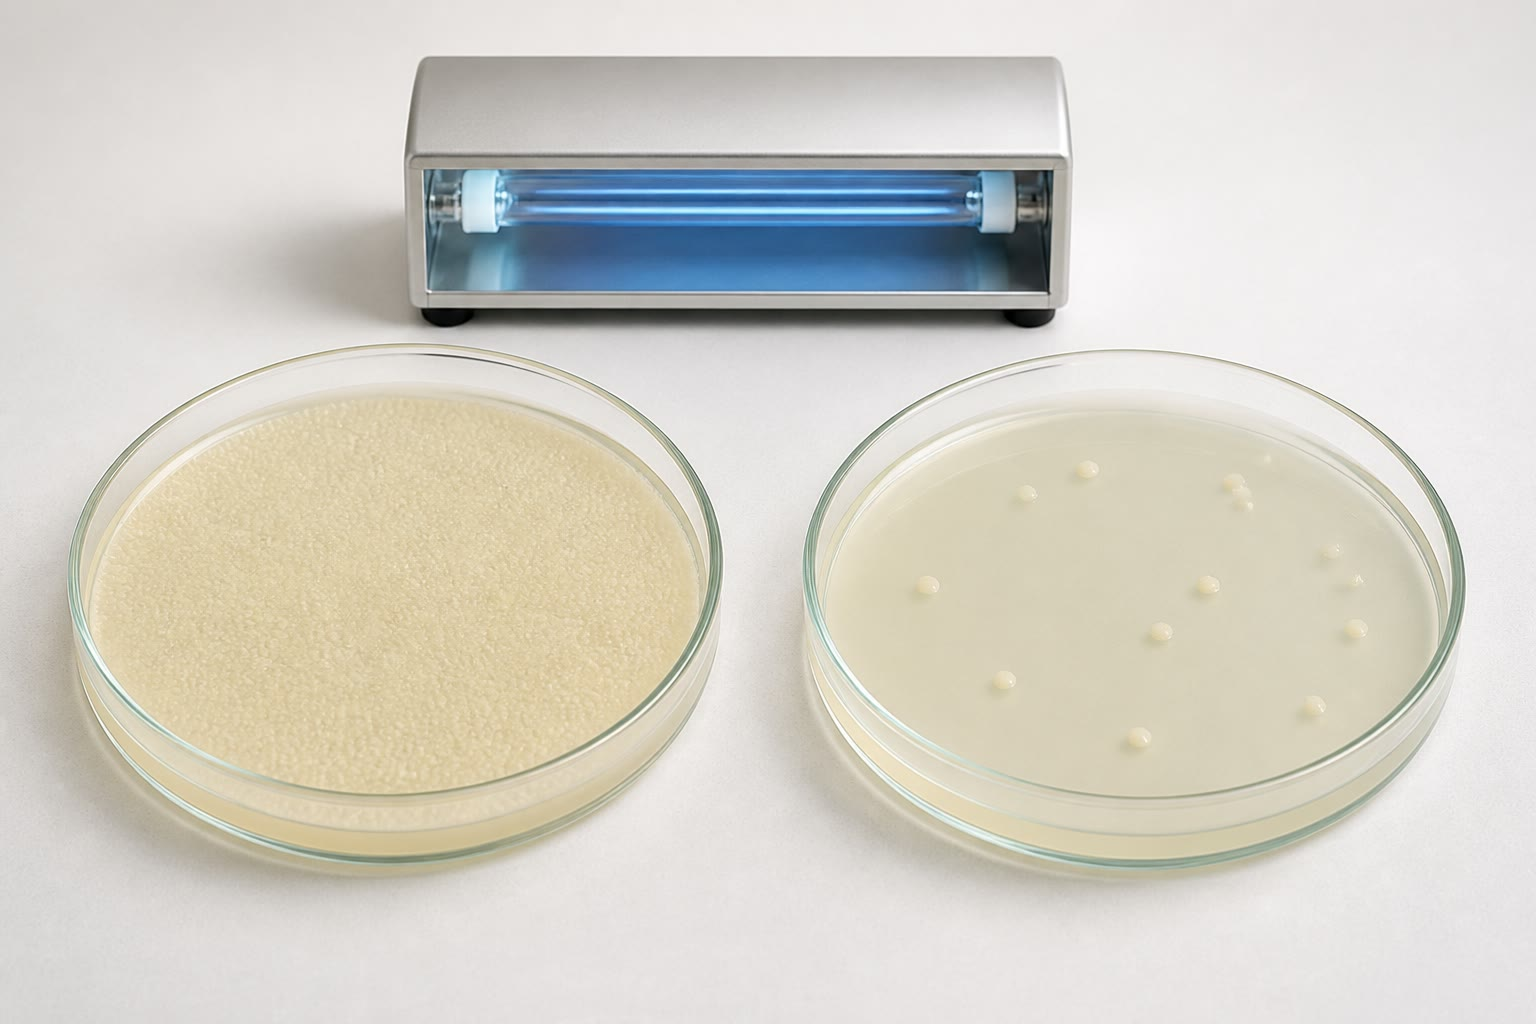
\includegraphics[width=0.6\linewidth]{images/book2/ai/g11-mutation-uv-plates.jpg}

{\small 两个平板接种了相同的细菌。左：未照射，
形成连续菌苔。右：经紫外线照射后，仅及时修复
\omterm{def:g10:universal-dna:information}{DNA} 损伤的\omterm{def:g10:cells-common-unit:cell}{细胞}长成了菌落。}
\end{omfigure}

\section{细胞的反击：修复}

\begin{proposition}[DNA 修复]\label{prop:g11:mutations:repair}
一个\omterm{def:g10:cells-common-unit:cell}{细胞}每天会遭受数以万计的 \omterm{def:g10:universal-dna:information}{DNA} 损伤，却几乎都能将其清除：
专门的酶系统沿\omterm{prop:g10:universal-dna:helix}{双螺旋}巡查，
识别受损或错配的碱基，切除一条链上有缺陷的片段，
并以另一条链为模板重新合成——这正是
\cref{ch:g10:universal-dna}中碱基\omterm{prop:g10:universal-dna:helix}{互补性}的再一次体现。一处损伤
只有在下一次复制将其拷贝之前仍未得到修复，才会变成\omterm{def:g11:mutations:mutation}{突变}。
修复作用使\omterm{def:g11:mutations:mutation}{突变}率为 $10^{-9}$
而非 $10^{-5}$。
\end{proposition}
\begin{proof}[证据]
患有遗传性疾病着色性干皮病的人，缺乏其中一种
切除紫外线损伤的酶。他们的皮肤暴露于普通日光下，
皮肤在从幼儿期起患癌症的频率就比正常皮肤高出一千倍，
若避免日晒，则与正常皮肤无异。
同样的紫外线，同样的损伤——但若无修复，损伤便会留存，
\omterm{def:g11:mutations:mutation}{突变}便在控制\omterm{def:g10:cells-common-unit:cell}{细胞}分裂的\omterm{def:g10:universal-dna:gene}{基因}中累积
（见\cref{ch:g11:cancer}）。酵母和细菌中缺失修复酶的菌株，
在实验室中同样表现出
高度敏感性。
\end{proof}

\begin{omfigure}
\begin{tikzpicture}[font=\small, >=Stealth,
  b/.style={draw, rounded corners, align=center, text width=2.6cm, minimum height=1.1cm}]
  \node[b, fill=omProp!15] (a) at (0,0) {紫外线使 \\ 相邻两个 T 焊接};
  \node[b, fill=omDef!12] (bx) at (3.4,0) {修复酶 \\ 识别结构扭曲};
  \node[b, fill=omDef!12] (c) at (6.8,0) {受损片段 \\ 从一条链上切除};
  \node[b, fill=omDef!12] (d) at (10.2,0) {以完整链为模板 \\ 补齐缺口};
  \draw[->] (a) -- (bx); \draw[->] (bx) -- (c); \draw[->] (c) -- (d);
  \node[b, fill=omThm!12] (e) at (3.4,-2.0) {复制将损伤 \\ 拷贝下来};
  \node[b, fill=omThm!12] (f) at (6.8,-2.0) {突变，从此 \\ 永久保留};
  \draw[->] (a.south) |- node[pos=0.25, left, font=\scriptsize, align=right] {未及时 \\ 修复时} (e.west);
  \draw[->] (e) -- (f);
\end{tikzpicture}

{\small 修复与复制的赛跑。被切除并以另一条链重建的损伤不留痕迹；
\omterm{prop:g11:dna-replication:forks}{复制叉}经过时仍然存在的损伤，
会被拷贝进序列并成为
\omterm{def:g11:mutations:mutation}{突变}。}
\end{omfigure}

\section{突变的后果}

\begin{proposition}[从序列到表型]\label{prop:g11:mutations:consequences}
\omterm{def:g11:mutations:mutation}{突变}将一个\omterm{def:g10:universal-dna:gene}{等位基因}变为新的\omterm{def:g10:universal-dna:gene}{等位基因}。其效应取决于
\omterm{def:g11:mutations:mutation}{突变}发生的位置，以及它对该\omterm{def:g10:universal-dna:gene}{基因}所编码\omterm{def:g10:chemistry-of-life:families}{蛋白质}的影响
（相关规则见\cref{ch:g11:gene-expression}）：
\begin{itemize}
  \item 不在任何\omterm{def:g10:universal-dna:gene}{基因}之内，或位于不改变
        \omterm{def:g10:chemistry-of-life:families}{蛋白质}的位置：\emph{无效应}——占绝大多数；
  \item 位于\omterm{def:g10:universal-dna:gene}{基因}之内、改变一个\omterm{def:g10:chemistry-of-life:families}{氨基酸}：\omterm{def:g10:chemistry-of-life:families}{蛋白质}
        功能略有不同、完全失效，或偶尔更好；
  \item 位于\omterm{def:g10:universal-dna:gene}{基因}之内、使信息移码或截短：通常得到
        不能正常发挥作用的\omterm{def:g10:chemistry-of-life:families}{蛋白质}。
\end{itemize}
改变后的\omterm{def:g10:chemistry-of-life:families}{蛋白质}是有害、中性还是有利，取决于
环境：同一个血红蛋白\omterm{def:g10:universal-dna:gene}{基因}的\omterm{def:g10:universal-dna:gene}{等位基因}，在无疟疾的地区是负担，
在有疟疾的地区则起保护作用。
\end{proposition}
\admitted

\begin{example}[色素丢失，色素保留]\label{ex:g11:mutations:pigment}
黑色素由一种酶合成。已知其\omterm{def:g10:universal-dna:gene}{基因}有数十种不同的
\omterm{def:g11:mutations:mutation}{突变}，每一种都使酶失去功能；
若某人携带两个这样的\omterm{def:g10:universal-dna:gene}{等位基因}，便会出现
本章开头所述的无色素状态。这些\omterm{def:g11:mutations:mutation}{突变}每一个都是随机发生的，
且各自只发生一次、发生在生殖\omterm{def:g10:cells-common-unit:cell}{细胞}中；只有当两名携带者
将各自的隐性\omterm{def:g10:universal-dna:gene}{等位基因}传给同一个孩子时，该性状才会显现。同一\omterm{def:g10:universal-dna:gene}{基因}的
另一种\omterm{def:g10:universal-dna:gene}{等位基因}使酶的活性略低，皮肤颜色因此较浅——
这种情况在数千年来一直生活于
高纬度地区的人群中很常见，色素稍少，皮肤便能在较弱的阳光下合成更多的维生素
D。
\end{example}

\begin{proposition}[突变，多样性的来源]\label{prop:g11:mutations:source}
每个\omterm{def:g10:universal-dna:gene}{基因}的每一个\omterm{def:g10:universal-dna:gene}{等位基因}，都源于某个较早\omterm{def:g10:universal-dna:gene}{等位基因}的\omterm{def:g11:mutations:mutation}{突变}。
\omterm{def:g11:mutations:mutation}{突变}是唯一能够产生新\omterm{def:g10:universal-dna:information}{遗传信息}的过程；
最后一年学习的有性重组，只是将\omterm{def:g11:mutations:mutation}{突变}已产生的\omterm{def:g10:universal-dna:information}{遗传信息}重新组合。
\omterm{def:g11:mutations:mutation}{突变}罕见、随机，对个体而言多为中性或有害，
但在世代延续中，它提供了
演化所依赖的变异，这种演化见
\cref{ch:g10:biodiversity-scales}。
\end{proposition}
\admitted

\begin{method}[分析突变]\label{met:g11:mutations:analyse}
\begin{enumerate}
  \item 将\omterm{def:g11:mutations:mutation}{突变}序列与原序列逐个碱基比较，
        并指出变化的类型（替换、插入，
        或缺失；涉及几个\omterm{def:g10:universal-dna:nucleotide}{核苷酸}）。
  \item 确定其位置：位于\omterm{def:g10:universal-dna:gene}{基因}之内还是之外；
        若在\omterm{def:g10:universal-dna:gene}{基因}之内，信息的阅读框是否发生移位。
  \item 确定其发生的\omterm{def:g10:cells-common-unit:cell}{细胞}：体\omterm{def:g10:cells-common-unit:cell}{细胞}（只影响一个个体的一种组织）
        或生殖\omterm{def:g10:cells-common-unit:cell}{细胞}（可以遗传）。
  \item 若\omterm{def:g11:mutations:mutation}{突变}速率异常，寻找原因（如\omterm{def:g11:mutations:mutagen}{诱变剂}暴露、修复缺陷）；
        否则归因于偶然。
  \item 依次在\omterm{def:g10:chemistry-of-life:families}{蛋白质}、\omterm{def:g10:cells-common-unit:cell}{细胞}层面判断后果，
        再到生物体与种群层面，且应按此顺序，
        并注明所处的环境。
\end{enumerate}
\end{method}

\begin{remark}[再谈随机性]\label{rem:g11:mutations:random}
“随机”并不意味着所有位点\omterm{def:g11:mutations:mutation}{突变}的概率相同——有些序列更易断裂——
也不意味着\omterm{def:g11:mutations:mutation}{突变}没有原因。它的含义是：\omterm{def:g11:mutations:mutation}{突变}的发生
与其是否对\omterm{def:g10:cells-common-unit:cell}{细胞}有利无关：影印平板上的耐药菌
并非由抗生素使其产生抗性，
也没有任何生物体能够
“决定”向有利方向\omterm{def:g11:mutations:mutation}{突变}。
选择在事后起导向作用；\omterm{def:g11:mutations:mutation}{突变}只提供变异。
\end{remark}

\section{练习}

\begin{exercise}[$\star$]\label{exo:g11:mutations:1}
定义\omterm{def:g11:mutations:mutation}{突变}，并说出点\omterm{def:g11:mutations:mutation}{突变}的三种类型。
\end{exercise}

\begin{exercise}[$\star$]\label{exo:g11:mutations:2}
将 \texttt{ATGCCTGAAT} 与以下\omterm{def:g11:mutations:mutation}{突变}序列
\texttt{ATGCCAGAAT}、\texttt{ATGCCTGAT} 和 \texttt{ATGCCTTGAAT} 进行比较，指出每个\omterm{def:g11:mutations:mutation}{突变}的类型。
\end{exercise}

\begin{exercise}[$\star$]\label{exo:g11:mutations:3}
体\omterm{def:g10:cells-common-unit:cell}{细胞}\omterm{def:g11:mutations:mutation}{突变}与生殖\omterm{def:g10:cells-common-unit:cell}{细胞}\omterm{def:g11:mutations:mutation}{突变}有何区别？
哪一种对遗传有重要意义？
\end{exercise}

\begin{exercise}[$\star$]\label{exo:g11:mutations:4}
说出三种\omterm{def:g11:mutations:mutagen}{诱变剂}，并说明其中一种对 \omterm{def:g10:universal-dna:information}{DNA} 造成的损伤。
\end{exercise}

\begin{exercise}[$\star$]\label{exo:g11:mutations:5}
修复系统以什么为模板重建受损的片段？
为什么这是可能的？
\end{exercise}

\begin{exercise}[$\star\star$]\label{exo:g11:mutations:6}
由存活率图可知，正常酵母
经 \qty{40}{s} 紫外线照射后的存活比例是多少？修复缺陷菌株的呢？
在该剂量下，修复使存活率提高了多少倍？
\end{exercise}

\begin{exercise}[$\star\star$]\label{exo:g11:mutations:7}
将 $10^9$ 个细菌的培养物涂布于抗生素平板上，
长出 20 个菌落。估算耐药\omterm{def:g10:cells-common-unit:cell}{细胞}的频率。
这能否说明该\omterm{def:g11:mutations:mutation}{突变}是由抗生素引起的？
\end{exercise}

\begin{exercise}[$\star\star$]\label{exo:g11:mutations:8}
请用自己的语言解释，为什么耐药菌落在影印平板上的位置完全相同，
这能证明\omterm{def:g11:mutations:mutation}{突变}是在
接触抗生素之前发生的。
\end{exercise}

\begin{exercise}[$\star\star$]\label{exo:g11:mutations:9}
某\omterm{def:g10:universal-dna:gene}{基因}长 \num{3000} 个碱基对，复制时每 $10^9$ 个\omterm{def:g10:universal-dna:nucleotide}{核苷酸}出现一处错误。
一个组织含 $10^{12}$ 个\omterm{def:g10:cells-common-unit:cell}{细胞}，全部由一个\omterm{def:g10:cells-common-unit:cell}{细胞}经 40 次分裂而来，
估算大约有多少个\omterm{def:g10:cells-common-unit:cell}{细胞}在该\omterm{def:g10:universal-dna:gene}{基因}上带有新\omterm{def:g11:mutations:mutation}{突变}？
（仅计算最后一次分裂中产生的错误。）
\end{exercise}

\begin{exercise}[$\star\star$]\label{exo:g11:mutations:10}
一株玫瑰的一根枝条开出了颜色不同的花。
用该枝条扦插，所得植株开出新颜色的花；
用其花上的种子培育，所得则是普通玫瑰。请解释这两种结果。
\end{exercise}

\begin{exercise}[$\star\star$]\label{exo:g11:mutations:11}
为什么患有着色性干皮病的人会发生皮肤癌，
而不会（例如）发生肠道癌？
\end{exercise}

\begin{exercise}[$\star\star\star$]\label{exo:g11:mutations:12}
防晒霜吸收紫外线。利用存活率图，解释
透过十分之一紫外线的防晒霜，会使
一小时日晒中每个皮肤\omterm{def:g10:cells-common-unit:cell}{细胞}的损伤数目发生什么变化，以及为何“没有晒伤”
并不等于“没有\omterm{def:g11:mutations:mutation}{突变}”。
\end{exercise}

\begin{exercise}[$\star\star\star$]\label{exo:g11:mutations:13}
血红蛋白\omterm{def:g10:universal-dna:gene}{基因}的一个\omterm{def:g10:universal-dna:gene}{等位基因}，在携带一份拷贝时
可抵御疟疾，但在携带两份拷贝时会引发严重疾病。讨论
该\omterm{def:g11:mutations:mutation}{突变}是“有害”还是“有益”，以及由什么因素决定。
\end{exercise}

\begin{exercise}[$\star\star\star$]\label{exo:g11:mutations:14}
细菌在不含抗生素的肉汤中培养，30
代后，发现每一百万个\omterm{def:g10:cells-common-unit:cell}{细胞}中有一个抗性\omterm{def:g10:cells-common-unit:cell}{细胞}。若随后加入
抗生素，培养物在一天之内会发生什么变化？
解释为什么医生要求必须完整服用一个疗程的抗生素。
\end{exercise}

\begin{exercise}[$\star\star\star$]\label{exo:g11:mutations:15}
“若\omterm{def:g11:mutations:mutation}{突变}几乎总是有害的，演化便不可能建立在
其上。”请用一段话讨论，运用随机性、
中性\omterm{def:g11:mutations:mutation}{突变}的比例、环境以及时间尺度等概念。
\end{exercise}

\section{问题：绒布印章}

\begin{problem}[{周末问题——重现莱德伯格的影印平板实验：
计数菌落、标出抗性、判定突变的来源，
并测定其速率}]
\label{pb:g11:mutations:1}
一名学生将约 200 个细菌（取自从未接触过链霉素的培养物）涂布
在不含抗生素的平板上。一夜之后，
长出 200 个菌落，每个菌落都来自一个\omterm{def:g10:cells-common-unit:cell}{细胞}，各含
约 $10^7$ 个\omterm{def:g10:cells-common-unit:cell}{细胞}。将绒布印章压在平板上，再盖印到
三块含链霉素的平板上。次日，A 平板出现
两个抗性菌落，B 平板两个，C 平板两个——
三块平板上的两个位置完全相同。

\medskip
\noindent\textbf{第一部分——实验。}
\begin{enumerate}
  \item 为什么原始平板上的菌落必须来自单个\omterm{def:g10:cells-common-unit:cell}{细胞}，
        且为何涂布的细菌数量要保持较少？
  \item 说明绒布印章转移了什么，以及为何菌落
        的位置能够保持不变。
  \item 200 个位置中有两个，在每一块复制
        平板上都长出抗性菌落。三块复制平板
        之间的一致性说明了什么？
  \item 假设抗生素是在接触时诱导少量\omterm{def:g10:cells-common-unit:cell}{细胞}产生
        抗性。描述三块复制平板会呈现的
        图样。
  \item 两种假设——接触前发生\omterm{def:g11:mutations:mutation}{突变}，与接触时诱导，
        哪一种为观察到的图样所支持？
        用一句话陈述论据。
\end{enumerate}

\medskip
\noindent\textbf{第二部分——回到原始平板。}
\begin{enumerate}[resume]
  \item 学生从两个抗性位置取\omterm{def:g10:cells-common-unit:cell}{细胞}，
        这些位置位于\emph{原始}平板上（该平板从未接触过抗生素），
        另从两个其他位置取样，将每份样品进行
        链霉素检验。预测结果。
  \item 两个抗性位置的菌落各含约
        $10^7$ 个\omterm{def:g10:cells-common-unit:cell}{细胞}。这些\omterm{def:g10:cells-common-unit:cell}{细胞}是全部具有抗性，
        还是仅部分具有抗性？要做出判断，需要知道什么？
  \item 一个菌落由单个\omterm{def:g10:cells-common-unit:cell}{细胞}经约 23 次分裂生长而来。若
        \omterm{def:g11:mutations:mutation}{突变}发生于第 20 次分裂，则该菌落中携带
        \omterm{def:g11:mutations:mutation}{突变}的\omterm{def:g10:cells-common-unit:cell}{细胞}占多大比例？若发生于第 3 次分裂呢？
  \item 解释为何检验整个菌落，
        能够发现仅发生于部分\omterm{def:g10:cells-common-unit:cell}{细胞}中的\omterm{def:g11:mutations:mutation}{突变}。
  \item 为什么只有当复制平板上的菌落
        \emph{恰好}长在原始菌落所在的位置上，
        实验才能成立？
\end{enumerate}

\medskip
\noindent\textbf{第三部分——测定速率。}
\begin{enumerate}[resume]
  \item 学生用 50 块原始平板重复实验，
        每块 200 个菌落，共 10\,000 个菌落，其中 30 个
        产生抗性复制结果。携带至少一个抗性\omterm{def:g10:cells-common-unit:cell}{细胞}的菌落
        占多大比例？
  \item 每个菌落由单个\omterm{def:g10:cells-common-unit:cell}{细胞}经约 $10^7$ 次
        \omterm{def:g10:cells-common-unit:cell}{细胞}分裂形成。估计一次给定的分裂产生抗性\omterm{def:g11:mutations:mutation}{突变}的
        概率。
  \item 链霉素抗性需要某一\omterm{def:g10:universal-dna:gene}{基因}中一个特定位置发生
        改变。将你的估计与每个\omterm{def:g10:universal-dna:nucleotide}{核苷酸}的复制错误率
        $10^{-9}$ 相比较，
        并加以评论。
  \item 由单个\omterm{def:g10:cells-common-unit:cell}{细胞}在不含抗生素的肉汤中培养出含
        $10^9$ 个\omterm{def:g10:cells-common-unit:cell}{细胞}的培养物。利用你测得的速率估计
        当抗生素最终加入时，该培养物可能含有多少个
        抗性\omterm{def:g10:cells-common-unit:cell}{细胞}。
  \item 若抗性\omterm{def:g11:mutations:mutation}{突变}发生在该培养物生长的早期，
        抗性\omterm{def:g10:cells-common-unit:cell}{细胞}的数目会如何变化？为何重复
        培养会得到差异很大的计数结果？
\end{enumerate}

\medskip
\noindent\textbf{第四部分——结果的意义。}
\begin{enumerate}[resume]
  \item 解释“\omterm{def:g11:mutations:mutation}{突变}是随机的”与
        “\omterm{def:g11:mutations:mutation}{突变}是罕见的”之间的区别，以及该实验
        确立了哪一个。
  \item 抗生素并未产生抗性。它对种群
        起了什么作用？
  \item 将本实验转译为
        \cref{prop:g11:mutations:source}的语言：
        是什么提供了变异，又是什么对其进行了筛选？
  \item 有学生反驳说，原始平板上的两个抗性菌落
        “看起来与其他菌落完全一样”。解释为何
        \omterm{def:g11:mutations:mutation}{突变}在环境改变之前可能是不可见的。
  \item 陈述结论：三块绒布复制平板上相同位置的结果
        证明了\omterm{def:g11:mutations:mutation}{突变}的来源，以及你所测得的
        每次分裂的\omterm{def:g11:mutations:mutation}{突变}速率。
\end{enumerate}
\end{problem}
